\Variant{24.05.2025 (1-smena)}
\QQ{1}{$a$, $b$ natural sonlar uçun $a\cdot b=2^3\cdot3^5\cdot7^2$ bölsa, EKUK$(a,\,b)$ ning eng kiçik qiymatini toping.
\Opts{$700$}{$504$}{$252$}{$756$}}
\QQ{2}{$[200;\,1\,000]$ kesmada $2$, $3$, $5$ va $7$ sonlariga bölganda qoldiq $1$ ga teng böladigan natural sonlar neçta?
\Opts{$3$ ta}{$4$ ta}{$2$ ta}{$5$ ta}}
\QQ{3}{Bir soat davomida Anvar $20$ ta, Sardor esa $21$ ta buyum tayyorlaydi. Agar ular bir xil miqdordagi detallar tayyorlaşi uçun, Anvar Sardordan $10$ minut köproq vaqt sarflagan bölsa, ularning har biri neçta detal tayyorlagan?
\Opts{$60$}{$70$}{$80$}{$90$}}
\QQ{4}{Sotuvçi $2$ xil mahsulotni $35\,000\,000$ sömga sotib, $40\%$ foyda qilgan. Agar birinçi mahsulotni $25\%$, ikkinçi mahsulotni $50\%$ foyda bilan sotgan bölsa, ikkinçi mahsulotning asl bahosini toping.
\Opts{$85\,000\,000$}{$21\,000\,000$}{$15\,000\,000$}{$10\,000\,000$}}
\QQ{5}{Soddalaştiring:
\[\frac{2^{98}+1}{2^{49}+2^{25}+1}\]
\Opts{$2^{50}-2^{24}+1$}{$2^{49}-2^{25}+1$}{$2^{49}+2^{25}+1$}{$2^{50}+2^{24}+1$}}
\QQ{6}{Hisoblang:
\[\frac1{\sqrt{7-\sqrt{24}}}-\frac1{\sqrt{7+\sqrt{24}}}\]
\Opts{$\dfrac25$}{$\dfrac15$}{$\dfrac52$}{$1$}}
\QQ{7}{Hisoblang:
\[\sqrt{2664^2-1776^2-888^2}\]
\Opts{$1774$}{$1776$}{$1777$}{$1778$}}
\QQ{8}{Agar arifmetik progressiyada $a_{98}=a_{99}$ va $a_{2n-1}+1=a_{3n+1}-2a_{n+1}+a_n$ bölsa, $a_1+a_2+a_3+\dots+a_{100}$ ning qiymatini toping.
\Opts{$100$}{$200$}{$-100$}{$-200$}}
\QQ{9}{$4x-x^2=C_1$ tenglamaning ildizlari $x_1$ va $x_2$ ga, $36x-x^2=C_2$ tenglamaning ildizlari $x_3$ va $x_4$ ga teng. Agar $x_1$, $x_2$, $x_3$ va $x_4$ sonlari ösuvçi geometrik progressiyani taşkil etsa, $\sqrt{C_1\cdot C_2}$ ni hisoblang.
\Opts{$9$}{$6$}{$27$}{$12$}}
\QQ{10}{Agar $2025^3-2023^3=a$ bölsa, $\sqrt{\dfrac{a-2}6}$ ning qiymatini toping.
\Opts{$2023$}{$2024$}{$2025$}{$2026$}}
\QQ{11}{Soddalaştiring:
\[\frac{\sqrt{xy}}{y\sqrt y-x\sqrt x}:\left(\frac1{\sqrt x}-\frac1{\sqrt y}\right)^{-1}\]
\Opts{$\dfrac1{x+\sqrt{xy}+y}$}{$\dfrac1{x-\sqrt{xy}-y}$}{$\dfrac1{x-\sqrt{xy}+y}$}{$-\dfrac1{x+\sqrt{xy}-y}$}}
\QQ{12}{Hisoblang:
\[\cos1125^\circ+\sin\frac{17\pi}6\]
\Opts{$\dfrac{\sqrt2+1}2$}{$\dfrac{\sqrt2-1}2$}{$\dfrac{\sqrt3+1}2$}{$\dfrac{\sqrt3-1}2$}}
\QQ{13}{Quyidagi tenglamaning $\left[-\dfrac{3\pi}2;\,\dfrac\pi4\right]$ oraliğidagi haqiqiy ildizlari sonini toping:
\[6\sin^2x-2\sin2x=5\]
\Opts{$2$ ta}{$3$ ta}{$4$ ta}{$5$ ta}}
\QQ{14}{Tengsizlikni yeçing:
\[x^2\cdot3^x+9>3^x+9x^2\]
\Opts{$(-1;\,1)\cup(2;\,\infty)$}{$[-1;\,1)\cup(2;\,\infty)$}{$[0;\,1)\cup(2;\,\infty)$}{$[-1;\,0)\cup(1;\,\infty)$}}
\QQ{15}{Tengsizlikni yeçing:
\[\log_{x-2}\left(x^2-4x+3\right)<\log_{x-2}1\]
\Opts{$(2;\,3)$}{$\left(3;\,2+\sqrt2\right)$}{$\left(2-\sqrt2;\,3\right)$}{$(1;\,3)$}}
\QQ{16}{Tenglamani yeçing:
\[\left|x^2-3\right|=5\]
\Opts{$2\sqrt2;\ -2\sqrt2$}{$2\sqrt2;\ \sqrt2$}{$\sqrt2;\ -2\sqrt2$}{$2;\ 4$}}
\QQ{17}{Tenglamalar sistemasidan $\dfrac{x+y}z$ ning qiymatini toping:
\[\begin{cases}(x+y)(x+y+z)=108,\\ (x+z)(x+y+z)=120,\\ (y+z)(x+y+z)=60\end{cases}\]
\Opts{$1$}{$2$}{$3$}{$0$}}
\QQ{18}{Tengsizlikning butun yeçimlari yiğindisini (agar u bitta bölsa, şu ildizini) toping:
\[\left|x^2-5x+2\right|\cdot\sqrt{10-3x-x^2}\le0\]
\Opts{$3$}{$2$}{$-3$}{$5$}}
\QQ{19}{Tengsizlikning butun yeçimlari yiğindisini toping:
\[\frac{2^{2x}-3\cdot2^{2x-1}+2}{x+4}>0\]
\Opts{$-1$}{$-2$}{$-6$}{$-10$}}
\QQ{20}{Agar $f(x)=3+\dfrac x{1+x}$ ga teng bölsa, $f^{-1}(x)$ ni toping. (Bu yerda $f^{-1}(x)$ — $f(x)$ funksiyaning teskari funksiyasi.)
\Opts{$\dfrac{3-x}{2+x}$}{$\dfrac{3-x}{1+x}$}{$\dfrac{3-x}{3+x}$}{$\dfrac{3-x}{x-4}$}}
\QQ{21}{$f(x)$ toq funksiya uçun $f(x)-x^2f(-x)=x^3+5x$ bölsa, $f(-1)$ ning qiymatini toping.
\Opts{$3$}{$-3$}{$1$}{$-1$}}
\QQ{22}{Agar $f(x)=\sqrt{x+2\sqrt{2x-4}}-\sqrt{x-2\sqrt{2x-4}}$ bölsa, $f'(6)$ ning qiymatini toping.
\Opts{$2$}{$0$}{$2\sqrt2$}{$-2$}}
\QQ{23}{Aniq integralni hisoblang:
\[\int_0^{\frac\pi4}\frac{\sin^6x}{\cos^8x}\,dx\]
\Opts{$\dfrac18$}{$\dfrac17$}{$\dfrac16$}{$\dfrac15$}}
\QQ{24}{Kvadratga aylana içki çizilgan. Kvadrat perimetrini aylana uzunligiga nisbatini toping.
\Opts{$\dfrac4\pi$}{$\dfrac2\pi$}{$\dfrac1\pi$}{$\dfrac\pi2$}}
\QQ{25}{$ABC$ uçburçakka markazi $O$ nuqtada bölgan aylana içki çizilgan. Agar $\angle AOB=150^\circ$, $AC=13$ va $BC=8$ bölsa, $ABC$ uçburçakning yuzini toping.
\qfig{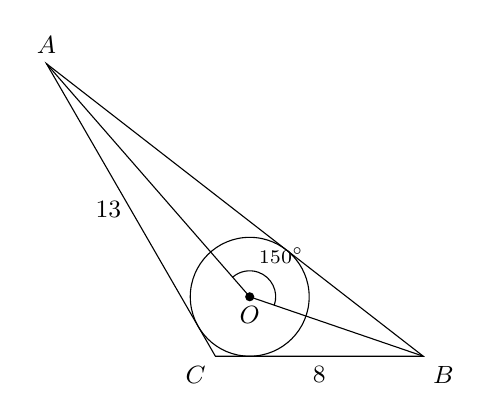
\begin{tikzpicture}[scale=0.33,font=\small]
\coordinate (C) at (0,0); \coordinate (B) at (8,0); \coordinate (A) at (-6.5,11.258); \coordinate (O) at (1.321,2.288);
\draw (A)--(B)--(C)--cycle; \draw (O) circle (2.288); \draw (A)--(O)--(B); \fill (O) circle (5pt);
\draw (O)+(-18.9:1) arc (-18.9:131.1:1);
\node[below left] at (C) {$C$}; \node[below right] at (B) {$B$}; \node[above] at (A) {$A$}; \node[below] at (O) {$O$};
\node[below] at (4,0) {$8$}; \node[left] at (-3.25,5.63) {$13$}; \node[above right] at (1.3,3.2) {\scriptsize$150^\circ$};
\end{tikzpicture}}
\Opts{$26\sqrt3$}{$26$}{$13\sqrt3$}{$13$}}
\QQ{26}{Quyidagi rasmda $ABC$ töğri burçakli uçburçak ($\angle B=90^\circ$) tasvirlangan. Agar $\angle BAD=\angle ACB$, $AD=10$ va $AC=15$ bölsa, $ABD$ uçburçak yuzining $ADC$ uçburçak yuziga nisbatini toping.
\qfig{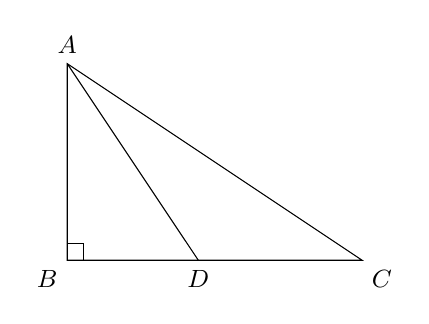
\begin{tikzpicture}[scale=0.3,font=\small]
\coordinate (B) at (0,0); \coordinate (A) at (0,8.32); \coordinate (D) at (5.547,0); \coordinate (C) at (12.48,0);
\draw (A)--(B)--(C)--cycle; \draw (A)--(D); \draw (0,0.7)--(0.7,0.7)--(0.7,0);
\node[above] at (A) {$A$}; \node[below left] at (B) {$B$}; \node[below] at (D) {$D$}; \node[below right] at (C) {$C$};
\end{tikzpicture}}
\Opts{$\dfrac35$}{$\dfrac45$}{$\dfrac75$}{$\dfrac25$}}
\QQ{27}{Quyidagi rasmda $ABCD$ va $DEFG$ kvadratlar tasvirlangan. Agar $AD=16$, $M$ va $N$ nuqtalar mos ravişda $GF$ va $BC$ tomonlarning örtalari bölsa, $ANM$ uçburçak yuzini toping.
\qfig{\begin{tikzpicture}[scale=0.17,font=\small]
\coordinate (A) at (0,0); \coordinate (D) at (16,0); \coordinate (C) at (16,16); \coordinate (B) at (0,16); \coordinate (N) at (8,16); \coordinate (G) at (16,8); \coordinate (F) at (24,8); \coordinate (E) at (24,0); \coordinate (M) at (20,8);
\fill[qfill] (A)--(N)--(M)--cycle;
\draw (A)--(B)--(C)--(D)--cycle; \draw (D)--(E)--(F)--(G); \draw (A)--(N)--(M)--cycle;
\node[below left] at (A) {$A$}; \node[above left] at (B) {$B$}; \node[above right] at (C) {$C$}; \node[below] at (D) {$D$}; \node[above] at (N) {$N$}; \node[above left] at (G) {$G$}; \node[above right] at (F) {$F$}; \node[below right] at (E) {$E$}; \node[above] at (M) {$M$};
\end{tikzpicture}}
\Opts{$256$}{$128$}{$64\sqrt2$}{$32\sqrt3$}}
\QQ{28}{Quyidagi rasmda $ABCDEFGH$ muntazam sakkizburçak tasvirlangan bölib, uning $HC$ va $BF$ diagonallari $K$ nuqtada kesişadi. $HKFG$ törtburçak yuzining $BKC$ uçburçak yuziga nisbati $\left(\dfrac{S_2}{S_1}\right)$ ni toping.
\qfig{\begin{tikzpicture}[scale=1.25,font=\small]
\coordinate (A) at (-0.5,1.207); \coordinate (B) at (0.5,1.207); \coordinate (C) at (1.207,0.5); \coordinate (D) at (1.207,-0.5); \coordinate (E) at (0.5,-1.207); \coordinate (F) at (-0.5,-1.207); \coordinate (G) at (-1.207,-0.5); \coordinate (H) at (-1.207,0.5); \coordinate (K) at (0.207,0.5);
\fill[qfill] (K)--(B)--(C)--cycle; \fill[qfill] (H)--(K)--(F)--(G)--cycle;
\draw (A)--(B)--(C)--(D)--(E)--(F)--(G)--(H)--cycle; \draw (H)--(C); \draw (B)--(F);
\node[above left] at (A) {$A$}; \node[above right] at (B) {$B$}; \node[right] at (C) {$C$}; \node[right] at (D) {$D$}; \node[below right] at (E) {$E$}; \node[below left] at (F) {$F$}; \node[left] at (G) {$G$}; \node[left] at (H) {$H$}; \node[below right] at (K) {$K$};
\node at (0.62,0.75) {$S_1$}; \node at (-0.8,0) {$S_2$};
\end{tikzpicture}}
\Opts{$\dfrac{3-\sqrt2}7$}{$\dfrac{3+\sqrt2}7$}{$\dfrac{3-\sqrt3}7$}{$3+\sqrt2$}}
\QQ{29}{Qavariq törtburçakning $A(0;\,0)$, $B(1;\,2)$, $C(3;\,3)$ va $D(4;\,0)$ uçlari bölsin. $DC$ tomonidan $E$ nuqta olingan, $AE$ kesma törtburçak yuzini teng ikkiga böladi. $E$ nuqtaning koordinatasini toping.
\Opts{$\left(\dfrac{17}5;\,\dfrac{15}7\right)$}{$\left(\dfrac{27}8;\,\dfrac{15}8\right)$}{$\left(\dfrac{15}8;\,\dfrac{15}7\right)$}{$\left(\dfrac{15}7;\,\dfrac{18}7\right)$}}
\QQ{30}{Muntazam törtburçakli piramida apofemasi asos tekisligi bilan $45^\circ$ burçak hosil qiladi. Agar yon sirt yuzi $144\sqrt2$ ga teng bölsa, piramida hajmini toping.
\Opts{$141$}{$72$}{$288$}{$36$}}
\QQ{31}{Quyidagi töplamlar berilgan, javoblardan qaysi biri $D\cup E$ ga aynan teng?
\[A=\{x\mid x\in\mathbb Z,\ 2\le x\le4\},\quad B=\{x\mid x\in\mathbb Z,\ 6\le x\le8\},\quad C=\{x\mid x\in\mathbb Z,\ 3\le x\le7\},\]
\[D=\{x\mid x\in\mathbb Z,\ 3\le x\le4\},\quad E=\{x\mid x\in\mathbb Z,\ 6\le x\le7\}\]
\Opts{$(A\cup B)\cap D$}{$(A\cup D)\cap C$}{$(A\cup B)\cap C$}{$(D\cup B)\cap E$}}
\QQ{32}{$5>a>b>c$ şartni qanoatlantiradigan $a$, $b$, $c$ raqamlardan eng köpi bilan neçta $\overline{abc}$ körinişidagi uç xonali sonlar tuziş mumkin?
\Opts{$8$ ta}{$9$ ta}{$10$ ta}{$7$ ta}}
\QQ{33}{\Moslash{Quyidagi rasmda diagonallari kesişgan nuqtasi $O$ bölgan $ABCDA_1B_1C_1D_1$ kub tasvirlangan. $M$ va $N$ nuqtalar mos ravişda $AD$ va $AB$ tomonlarining örtasida joylaşgan.
\par\centering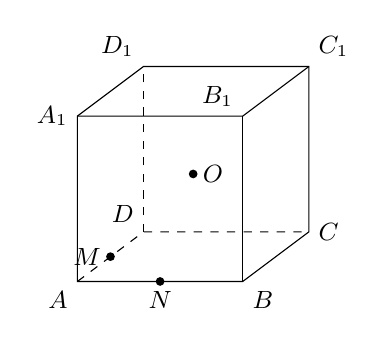
\begin{tikzpicture}[scale=1.05,font=\small]
\coordinate (A) at (0,0); \coordinate (B) at (2,0); \coordinate (C) at (2.8,0.6); \coordinate (D) at (0.8,0.6);
\coordinate (A1) at (0,2); \coordinate (B1) at (2,2); \coordinate (C1) at (2.8,2.6); \coordinate (D1) at (0.8,2.6);
\coordinate (M) at (0.4,0.3); \coordinate (N) at (1,0); \coordinate (O) at (1.4,1.3);
\draw (A)--(B)--(C)--(C1)--(D1)--(A1)--cycle; \draw (A1)--(B1)--(C1); \draw (B)--(B1);
\draw[dashed] (A)--(D)--(C); \draw[dashed] (D)--(D1);
\fill (M) circle (1.5pt); \fill (N) circle (1.5pt); \fill (O) circle (1.5pt);
\node[below left] at (A) {$A$}; \node[below right] at (B) {$B$}; \node[right] at (C) {$C$}; \node[above left] at (D) {$D$};
\node[left] at (A1) {$A_1$}; \node[above left] at (B1) {$B_1$}; \node[above right] at (C1) {$C_1$}; \node[above left] at (D1) {$D_1$};
\node[left] at (M) {$M$}; \node[below] at (N) {$N$}; \node[right] at (O) {$O$};
\end{tikzpicture}}{A) $\dfrac{\sqrt{15}}5$\par B) $\dfrac{\sqrt{15}}4$\par C) $\dfrac35$\par D) $\dfrac{\sqrt3}2$\par E) $\dfrac45$\par F) $\dfrac{\sqrt{10}}5$}{$MON$ burçak sinusini toping.}{$MD_1O$ burçak kosinusini toping.}{$MCN$ burçak kosinusini toping.}}
\QQ{36}{Quyidagi tenglama berilgan:
\[\left(x^3+3\right)^3=64(4x-3)\]
\AB{Tenglama neçta haqiqiy ildizga ega?}{Tenglamaning özaro teng bölmagan haqiqiy ildizlari yiğindisini toping.}}
\QQ{37}{Tenglamani yeçing:
\[x^2+4x\cos(xy)+4=0\]
Bunda $xy\in[-\pi;\,\pi]$.
\AB{Tenglamani qanoatlantiruvçi $(x;\,y)$ juftliklar neçta?}{$x+y$ ning eng kiçik qiymatini toping.}}
\QQ{38}{$f(x)$ funksiya uçun $2f(x)+3f(-1)+f\left(\dfrac1x\right)=x$ tenglik örinli.
\AB{$f(1)$ ning qiymatini toping.}{Agar $f(x)=1$ tenglamaning ildizlari $x_1$ va $x_2$ bölsa, $\dfrac1{x_1^2}+\dfrac1{x_2^2}$ ning qiymatini toping.}}
\QQ{39}{$y=f(x)$ funksiya va uning $x=1$ nuqtasiga ötkazilgan $y=kx+l$ urinma tenglamasi berilgan.
\qfig{\begin{tikzpicture}[x=1.1cm,y=0.75cm,font=\small]
\draw[-{Stealth[length=4pt]}] (-0.6,0)--(3.6,0) node[right] {$x$}; \draw[-{Stealth[length=4pt]}] (0,-0.9)--(0,3.6) node[left] {$y$};
\draw[thick] plot[smooth,tension=0.7] coordinates {(-0.1,0.9) (0.2,1.85) (0.55,2.25) (1,2) (1.5,1.2) (2,0.5) (2.4,0.15)};
\draw (-0.3,3.3)--(3.3,-0.3);
\draw[dashed] (0,2)--(1,2)--(1,0); \fill (1,2) circle (2pt);
\node[left] at (0,2) {$2$}; \node[below] at (1,0) {$1$}; \node[below] at (3,0) {$3$}; \node[below left] at (0,0) {$O$};
\node[right] at (0.6,3.1) {$y=kx+l$}; \node[below] at (2.4,-0.3) {$y=f(x)$};
\end{tikzpicture}}
\AB{$f'(1)$ ni toping.}{$h(x)=\left(x^3-2x^2+x+3\right)\cdot f(x)$ bölsa, $h'(1)$ ni toping.}}
\QQ{40}{Quyidagi rasmda $(-8;\,5)$ oraliqda $y=f(x)$ funksiya grafigi tasvirlangan.
\qfig{\begin{tikzpicture}[x=0.42cm,y=0.42cm,font=\small]
\draw[-{Stealth[length=4pt]}] (-9,0)--(6.3,0) node[right] {$x$}; \draw[-{Stealth[length=4pt]}] (0,-3)--(0,7.3) node[left] {$y$};
\draw[thick] plot[smooth,tension=0.6] coordinates {(-8,1.5) (-6.5,3.3) (-4,4) (-2.6,1.6) (-1.6,-1.3) (-1,-2) (-0.45,-1.4) (0,0) (1,3.4) (2,5.5) (3,6) (4,4.6) (5,1.5)};
\draw[dashed] (-8,0)--(-8,1.5); \draw[dashed] (-4,0)--(-4,4)--(0,4); \draw[dashed] (-1,0)--(-1,-2)--(0,-2); \draw[dashed] (3,0)--(3,6)--(0,6); \draw[dashed] (5,0)--(5,1.5);
\node[below] at (-8,0) {$-8$}; \node[below] at (-4,0) {$-4$}; \node[above] at (-1,0) {$-1$}; \node[below] at (3,0) {$3$}; \node[below] at (5,0) {$5$};
\node[right] at (0,4) {$4$}; \node[left] at (0,6) {$6$}; \node[right] at (0,-2) {$-2$}; \node[right] at (3.6,6) {$y=f(x)$};
\end{tikzpicture}}
\AB{$\displaystyle\int_{-4}^3\left(\left|f'(x)\right|-f'(x)\right)dx$ ni hisoblang.}{$\displaystyle\int_{-4}^3\left(f(x)+f'(x)\cdot x+f(x)\cdot f'(x)\right)dx$ ni hisoblang.}}
\QQ{41}{Quyidagi rasmda ikkita uçi aylanada joylaşgan $ABC$ uçburçak tasvirlangan: $A$ va $B$ aylanada, $BC$ — aylanaga $B$ nuqtada urinma, $AC$ tomon aylanani $D$ nuqtada kesadi. Bunda $AB=3$, $BD=2$ va $AD=3$.
\qfig{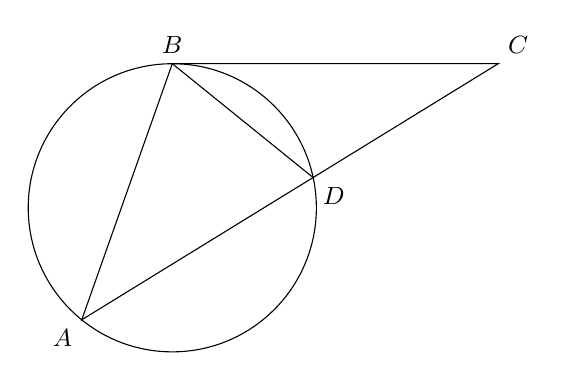
\begin{tikzpicture}[scale=1.15,font=\small]
\coordinate (B) at (0,1.591); \coordinate (D) at (1.555,0.334); \coordinate (A) at (-1.0,-1.237); \coordinate (C) at (3.599,1.591);
\draw (0,0) circle (1.591); \draw (A)--(B)--(C)--cycle; \draw (B)--(D);
\node[above] at (B) {$B$}; \node[below right] at (D) {$D$}; \node[below left] at (A) {$A$}; \node[above right] at (C) {$C$};
\end{tikzpicture}}
\AB{$BDC$ uçburçak yuzini toping.}{Aylana radiusini toping.}}
\QQ{42}{Uşbu rasmda $ABCD$ kvadrat tasvirlangan. $ABC$ uçburçak içida $E$ nuqta şunday joylaşganki, bunda $AE=2\sqrt3$, $BE=2\sqrt3$ va $EC=2\sqrt5$ ga teng.
\qfig{\begin{tikzpicture}[scale=0.62,font=\small]
\coordinate (A) at (0,0); \coordinate (B) at (5.565,0); \coordinate (C) at (5.565,5.565); \coordinate (D) at (0,5.565); \coordinate (E) at (2.783,2.064);
\fill[qfill] (A)--(E)--(C)--cycle;
\draw (A)--(B)--(C)--(D)--cycle; \draw (A)--(C); \draw (A)--(E)--(C); \draw (E)--(B);
\node[below left] at (A) {$A$}; \node[below right] at (B) {$B$}; \node[above right] at (C) {$C$}; \node[above left] at (D) {$D$}; \node[below] at (E) {$E$};
\end{tikzpicture}}
\AB{$ABCD$ kvadrat yuzini toping.}{$ACE$ uçburçakning yuzini toping.}}
\QQ{43}{Quyidagi rasmda $ABCDEFGH$ muntazam sakkizburçak tasvirlangan. $K$ nuqta $AD$ töğri çiziqda yotadi, $HK=12$ va $\angle KHG=60^\circ$.
\qfig{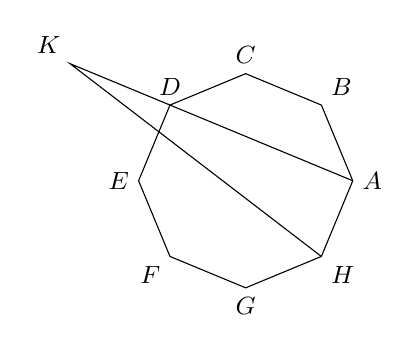
\begin{tikzpicture}[scale=0.85,font=\small]
\coordinate (A) at (1.6,0); \coordinate (B) at (1.131,1.131); \coordinate (C) at (0,1.6); \coordinate (D) at (-1.131,1.131); \coordinate (E) at (-1.6,0); \coordinate (F) at (-1.131,-1.131); \coordinate (G) at (0,-1.6); \coordinate (H) at (1.131,-1.131); \coordinate (K) at (-2.623,1.749);
\draw (A)--(B)--(C)--(D)--(E)--(F)--(G)--(H)--cycle; \draw (A)--(K)--(H);
\node[right] at (A) {$A$}; \node[above right] at (B) {$B$}; \node[above] at (C) {$C$}; \node[above] at (D) {$D$}; \node[left] at (E) {$E$}; \node[below left] at (F) {$F$}; \node[below] at (G) {$G$}; \node[below right] at (H) {$H$}; \node[above left] at (K) {$K$};
\end{tikzpicture}}
\AB{Muntazam sakkizburçakning tomoni uzunligini aniqlang.}{$AKH$ uçburçak yuzini toping.}}
\QQ{44}{Muntazam uçburçakli kesik piramidaning içiga şar içki çizilgan. Asoslarining yuzlari $9\sqrt3$ va $36\sqrt3$ ga teng.
\AB{Kesik piramidaning yon sirt yuzini toping.}{Şar sirtining yuzini toping (bunda $\pi=3$ deb oling).}}
\QQ{45}{Quyidagi rasmda barça qirralari $4$ cm ga teng bölgan $EABCD$ muntazam törtburçakli piramida tasvirlangan. $AE$ qirraning örtasi $F$ nuqtada turgan çumoli piramidaning sirti böylab $C$ nuqtaga bormoqçi.
\qfig{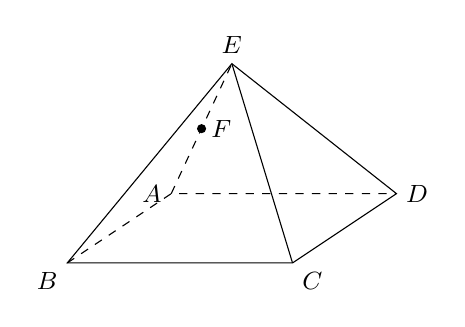
\begin{tikzpicture}[scale=1.1,font=\small]
\coordinate (B) at (0,0); \coordinate (C) at (2.6,0); \coordinate (D) at (3.8,0.8); \coordinate (A) at (1.2,0.8); \coordinate (E) at (1.9,2.3); \coordinate (F) at (1.55,1.55);
\draw (B)--(C)--(D)--(E)--cycle; \draw (E)--(C); \draw[dashed] (B)--(A)--(D); \draw[dashed] (A)--(E); \fill (F) circle (1.5pt);
\node[below left] at (B) {$B$}; \node[below right] at (C) {$C$}; \node[right] at (D) {$D$}; \node[left] at (A) {$A$}; \node[above] at (E) {$E$}; \node[right] at (F) {$F$};
\end{tikzpicture}}
\AB{Çumoli $F$ nuqtadan $C$ nuqtaga eng qisqa qança masofa bosib ötadi? (cm)}{Agar çumoli har $2$ daqiqada $\sqrt7$ cm masofa bosib ötsa, $F$ dan $C$ gaça neça daqiqa sarflaydi?}}
\Javoblar{D B B C B A B C C B A A B A B A C C C D B B B A A B B D B C C C D A E}{%
\OK{36}{$3$}{$0$}\OK{37}{$3$}{$-2$}\OK{38}{$\dfrac12$}{$\dfrac{41}4$}\OK{39}{$-1$}{$-3$}\OK{40}{$12$}{$44$}%
\OK{41}{$\dfrac{8\sqrt2}5$}{$\dfrac{9\sqrt2}8$}\OK{42}{$4\left(4+\sqrt{14}\right)$}{$2$}\OK{43}{$6\sqrt{2-\sqrt3}$}{$18$}\OK{44}{$81\sqrt3$}{$72$}\OK{45}{$2\sqrt7$}{$4$}}
